%!TeX root = Dissertation-DonaldDuck.tex
\chapter{Analyse}\label{cha:Analyse}

\blindtext[5]

\begin{figure}
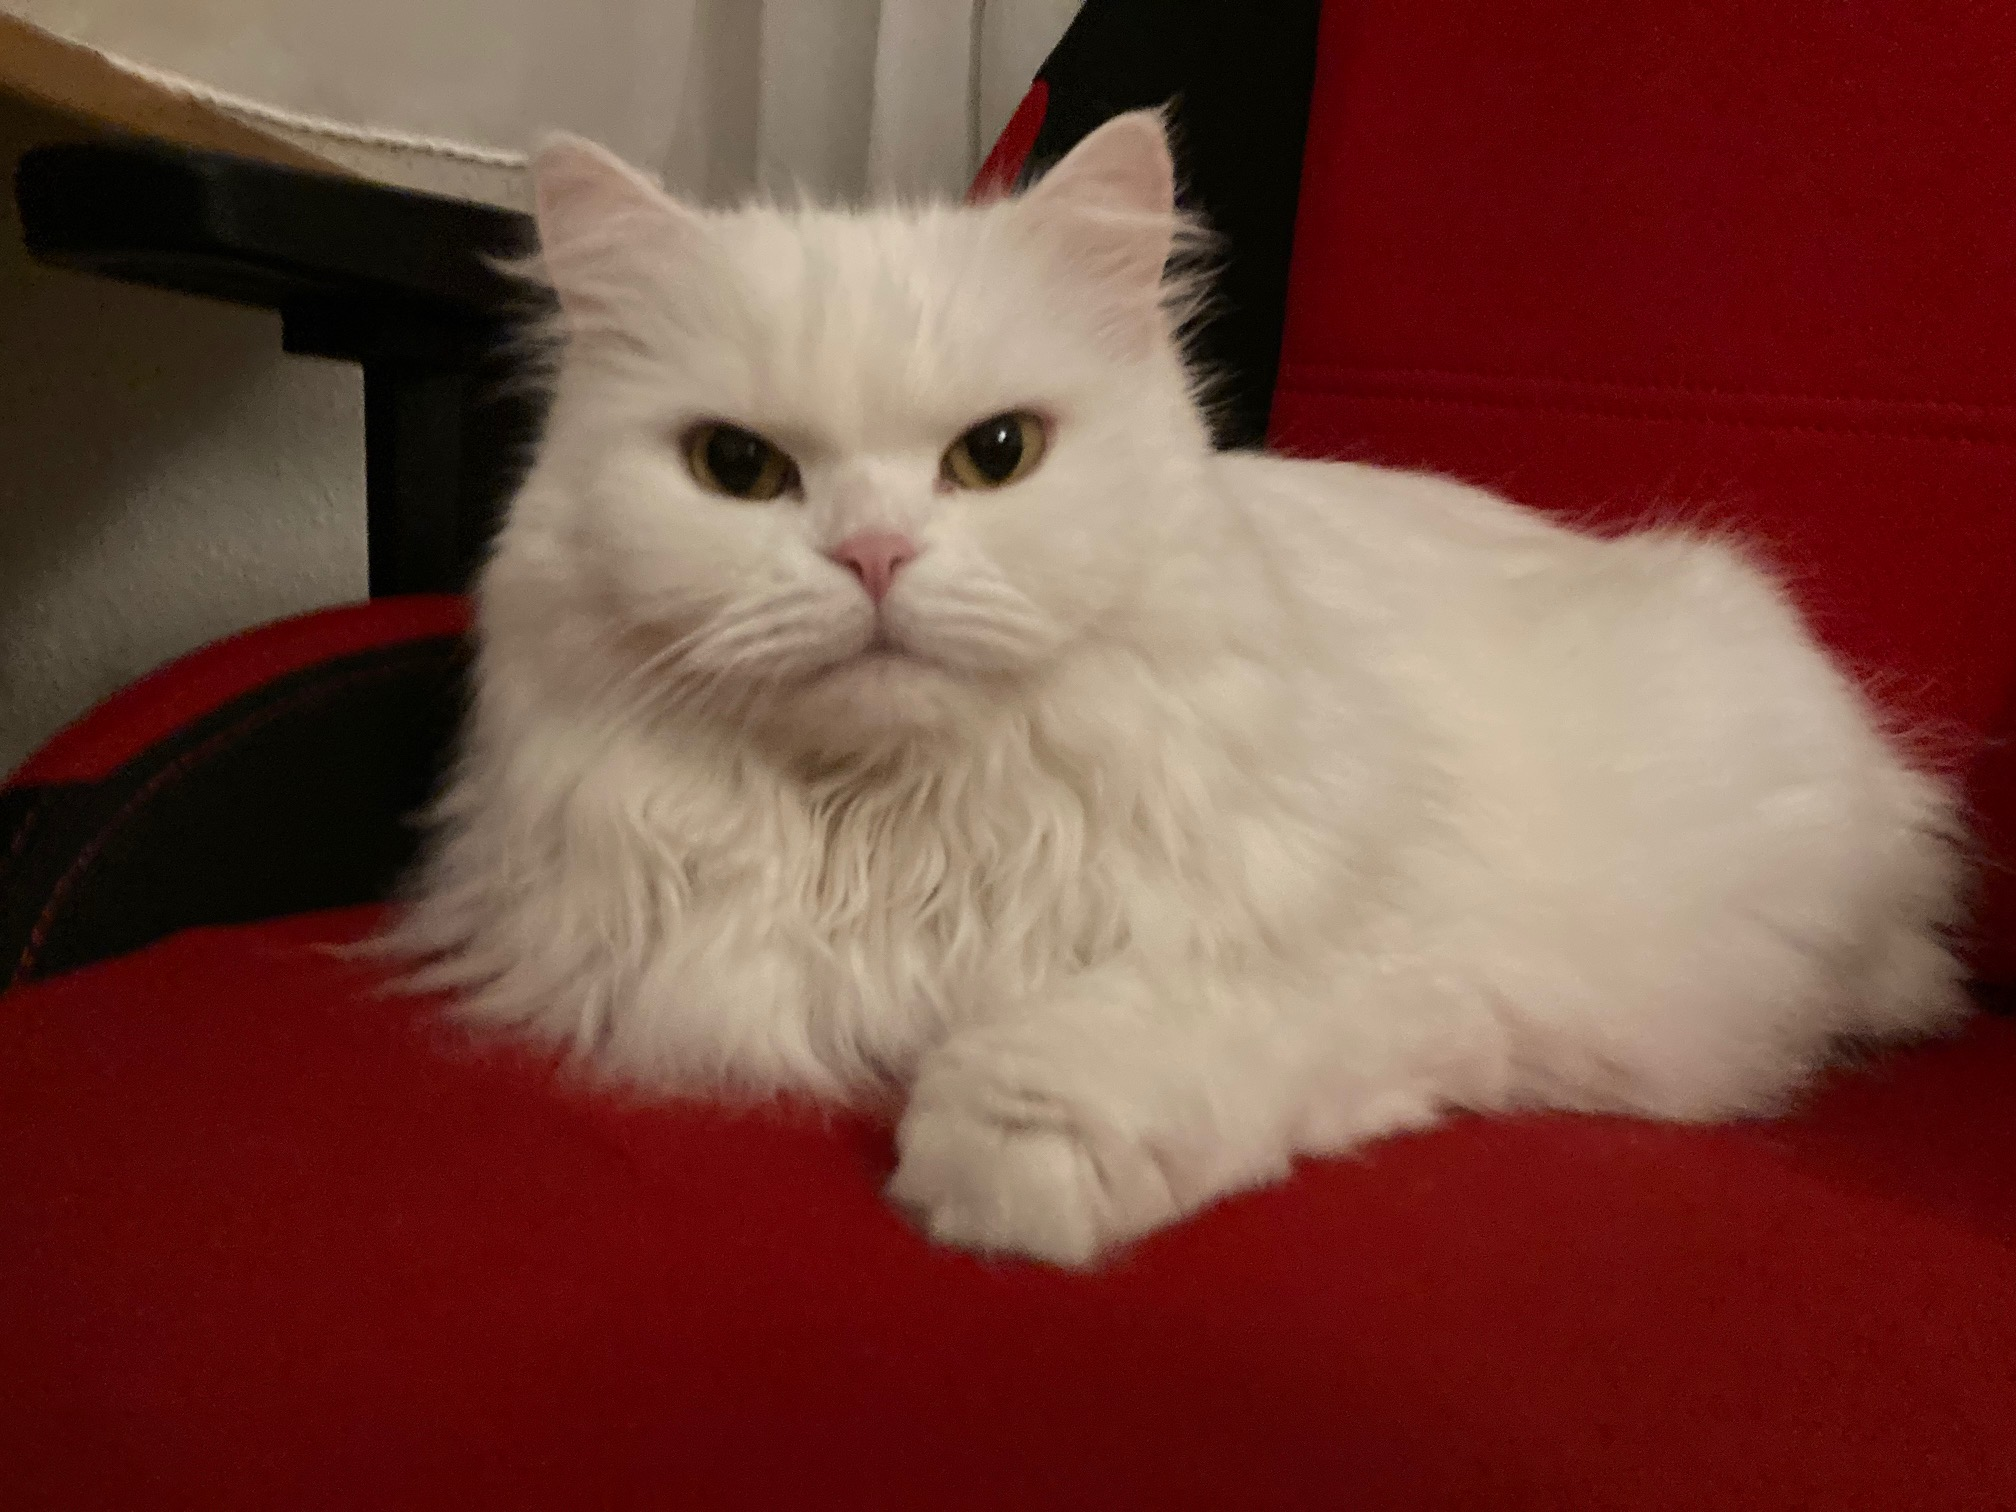
\includegraphics[width=\textwidth]{Bilder/Katze}
\caption{Meine Katze}\label{fig:Katze}
\end{figure}

\blindtext[5]

% Alternative zum Float
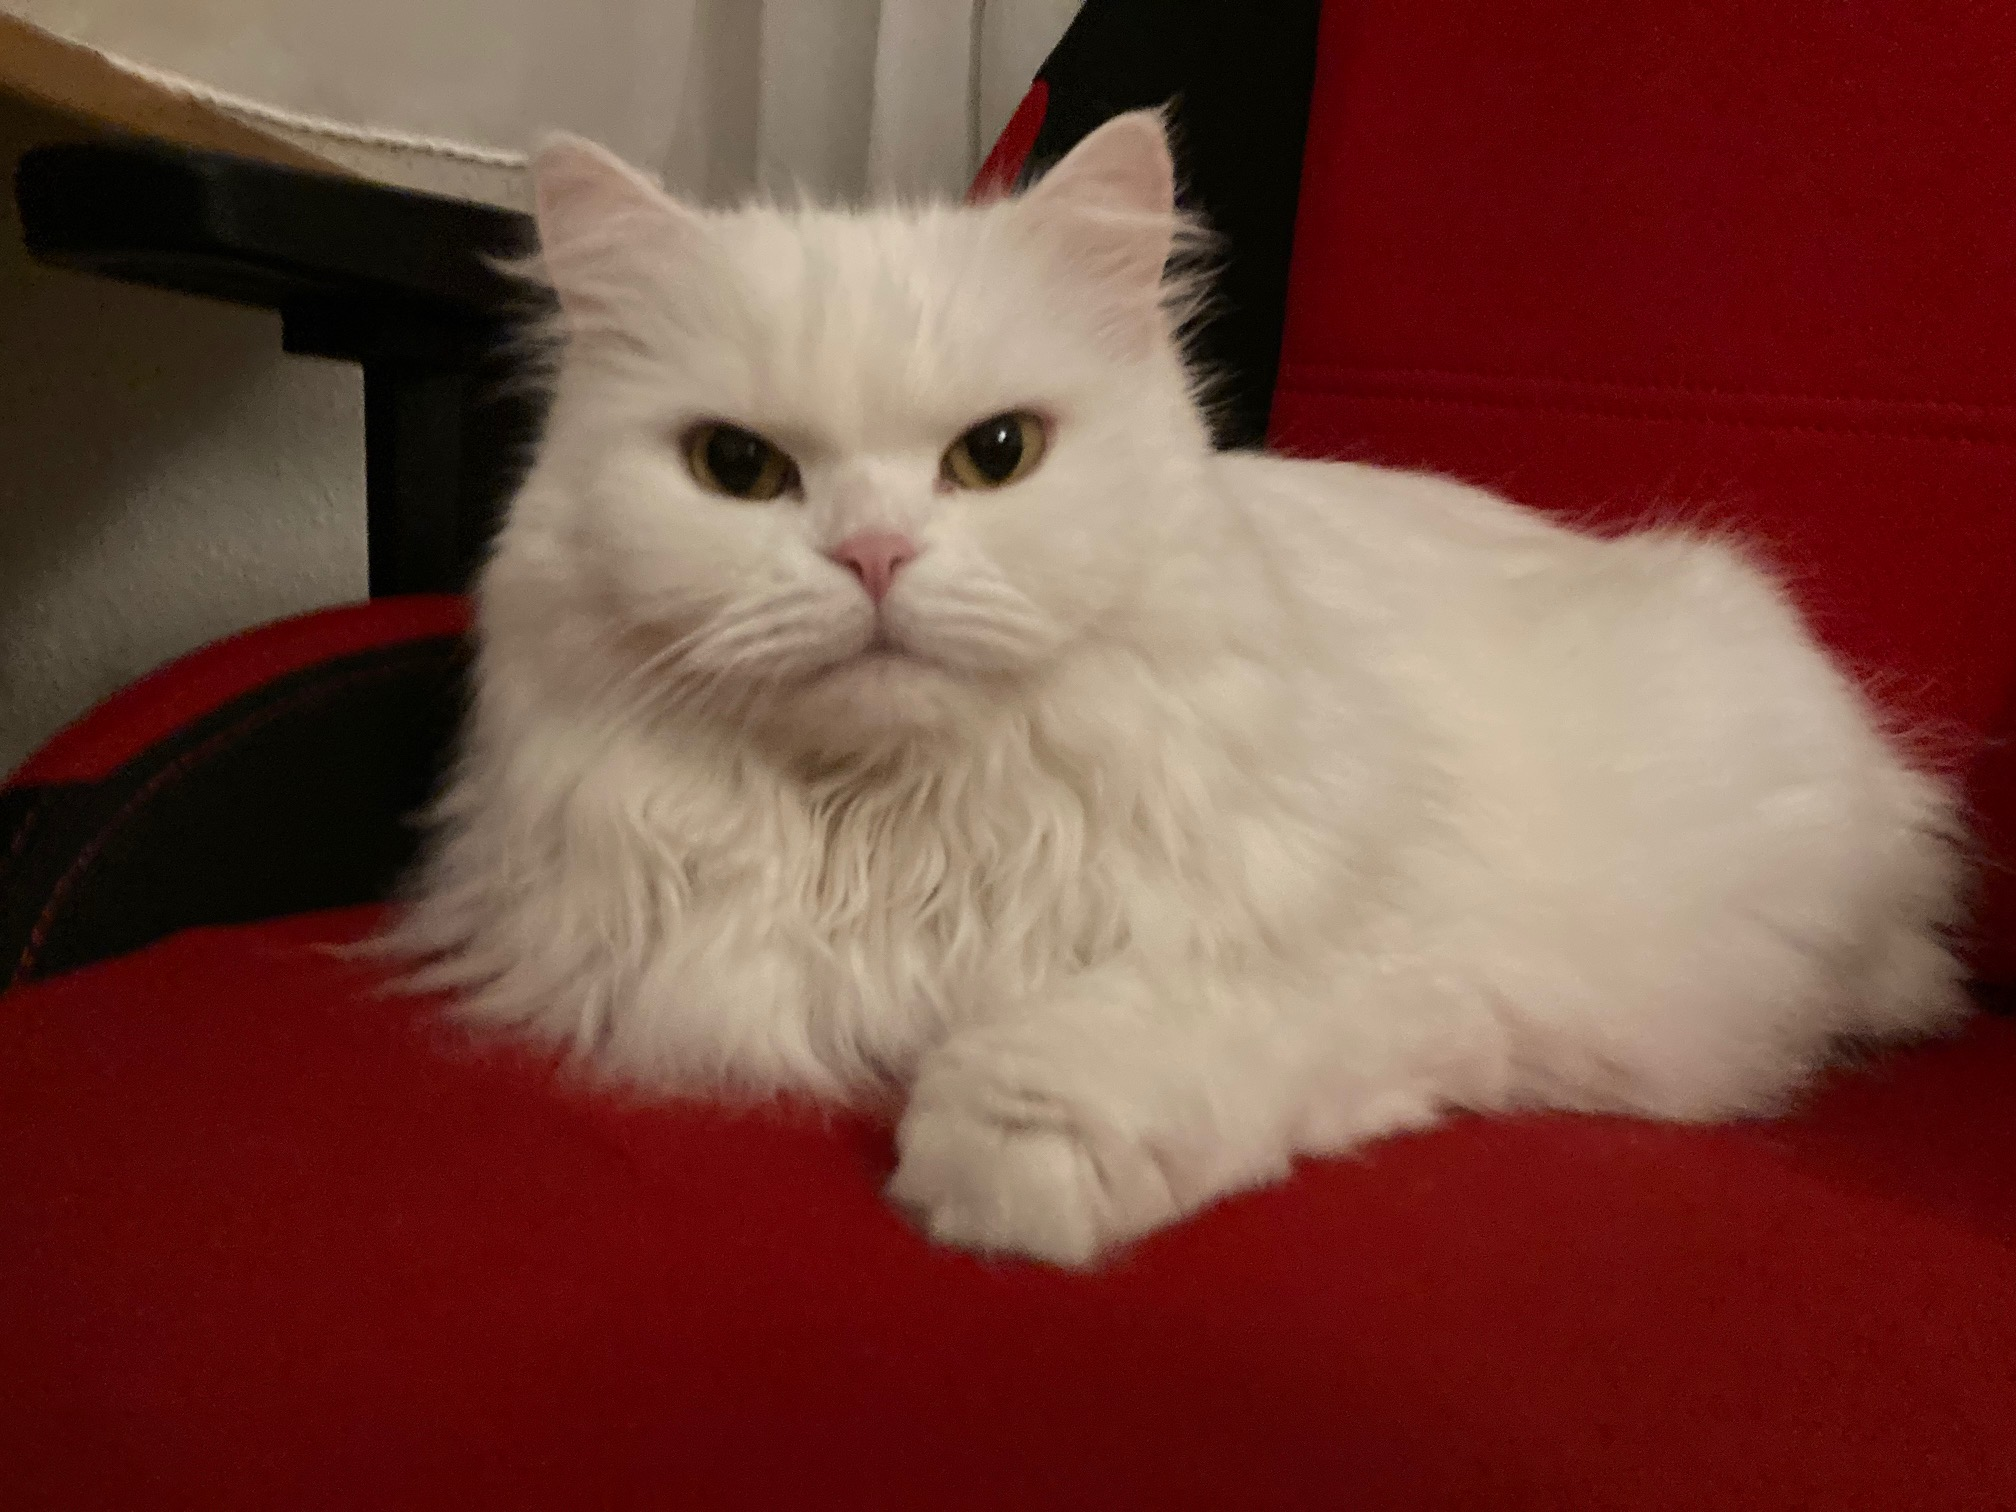
\includegraphics[width=\textwidth]{Bilder/Katze}
\captionof{figure}{Meine Katze 2}\label{fig:Katze2}

\blindtext[12]

\blindtext[12]

\blindtext[12]

\blindtext[12]